%=========== ΛΥΣΗ - 7ο ΘΕΜΑ Β ===========
\begin{thema}{Β}
Για κάθε $x\in\mathbb{R}$ είναι
\[f'(x)=\left[(x-a)e^x+1\right]'=(x-a)'e^x+(x-a)(e^x)'=e^x+(x-a)e^x=e^x(x-a+1)\]
\begin{erwthma}
\item Η $f$ παρουσιάζει τοπικό ακρότατο στο $x_0=1$ στο οποίο είναι και παραγωγίσιμη. Σύμφωνα λοιπόν με το θεώρημα \eng{Fermat} θα είναι \[f'(1)=0\Rightarrow e(1-a+1)=0\Rightarrow 2-a=0\Rightarrow a=2\]
οπότε $f(x)=(x-2)e^x+1$ και $f'(x)=e^x(x-1)\ ,\ x\in\mathbb{R}$.
\item Βρίσκουμε ρίζες και πρόσημα της $f'$:
\begin{itemize}
\item $f'(x)=0\Leftrightarrow e^x(x-1)=0\Leftrightarrow x-1=0\Leftrightarrow x=1$
\item $f'(x)>0\Leftrightarrow e^x(x-1)>0\Leftrightarrow x-1>0\Leftrightarrow x>1$
\item $f'(x)<0\Leftrightarrow e^x(x-1)<0\Leftrightarrow x-1<0\Leftrightarrow x<1$
\end{itemize}
Στον παρακάτω πίνακα βλέπουμε τα πρόσημα της $f'$ και τη μονοτονία της $f$
\begin{center}
\begin{tikzpicture}
\tkzTabInit[color,lgt=2,espcl=1.5,colorC = maincolor!50!white,colorL = maincolor!20!white,colorV = maincolor!50!white]%
{$x$ / .8,$f'(x)$ /0.8,$f(x)$/0.8}%
{$-\infty$,$1$,$+\infty$}%
\tkzTabLine{ , -, z, +, }
\tkzTabLine{ , \searrow,t ,\nearrow,}
\end{tikzpicture}
\end{center}
Βλέπουμε λοιπόν ότι
\begin{itemize}
\item η $f$ είναι \textbf{γνησίως φθίνουσα} στο διάστημα $\varDelta_1=(-\infty,1]$ άρα $f(\varDelta_1)=\left[f(1),\lim\limits_{x\to -\infty}{f(x)}\right)$
\begin{itemize}
\item $f(1)=(1-2)e^1+1=1-e$
\item $\lim\limits_{x\to-\infty}{f(x)}=\lim\limits_{x\to -\infty}{\left[(x-2)e^x+1\right]}\stackrel{0\cdot (-\infty)}{=}\lim\limits_{x\to -\infty}{\left(\dfrac{x-2}{e^{-x}}+1\right)}\xlongequal[\text{\eng{DLH}}]{\dfrac{-\infty}{+\infty}}$$\lim\limits_{x\to-\infty}{\left(-\dfrac{1}{e^{-x}}+1\right)}=0+1=1$
\end{itemize}
άρα $f(\varDelta_1)=[1-e,1)$. Παρατηρούμε ότι $0\in f(\varDelta_1)$ άρα η $f$ έχει μια τουλάχιστον ρίζα στο $\varDelta_1$ η οποία είναι μοναδική καθώς $f\searrow\varDelta_1$. Επίσης

\item η $f$ είναι \textbf{γνησίως αύξουσα} στο διάστημα $\varDelta_2=[1,+\infty)$ άρα $f(\varDelta_2)=\left[f(1),\lim\limits_{x\to +\infty}{f(x)}\right)=[1-e,+\infty)$ αφού
\[\lim\limits_{x\to+\infty}{f(x)}=\lim\limits_{x\to -\infty}{\left[(x-2)e^x+1\right]}=+\infty+1=+\infty\]
Παρατηρούμε ότι $0\in f(\varDelta_2)$ άρα η $f$ έχει μια τουλάχιστον ρίζα στο $\varDelta_2$ η οποία είναι μοναδική καθώς $f\nearrow\varDelta_2$.
\end{itemize}
Επομένως η $f$ έχει ακριβώς $2$ ρίζες.
\item Για κάθε $x\in\mathbb{R}$ είναι:
\[f''(x)=\left[e^x(x-1)\right]'=(e^x)'(x-1)+e^x(x-1)'=e^x(x-1)+e^x=xe^x\]
\begin{itemize}
\item $f''(x)=0\Leftrightarrow xe^x=0\Leftrightarrow x=0$
\item $f''(x)>0\Leftrightarrow xe^x>0\Leftrightarrow x>0$
\item $f''(x)<0\Leftrightarrow xe^x<0\Leftrightarrow x<0$
\end{itemize}
Στον παρακάτω πίνακα βλέπουμε την κυρτότητα της $f$ καθώς και τα σημεία καμπής της $C_f$:
\begin{center}
\begin{tikzpicture}
\tkzTabInit[color,lgt=2,espcl=1.5,colorC = maincolor!50!white,colorL = maincolor!20!white,colorV = maincolor!50!white]%
{$x$ / .8,$f''(x)$ /0.8,$f(x)$/0.8}%
{$-\infty$,$0$,$+\infty$}%
\tkzTabLine{ , -, z, +, }
\tkzTabLine{ ,\curvearrowright,t ,\rotatebox[origin= c]{180}{$\curvearrowleft$}, }
\end{tikzpicture}
\end{center}
H $f$ είναι κοίλη στο διάστημα $(-\infty,0]$ και κυρτή στο $[0,+\infty)$. Επιπλέον η $C_f$ έχει σημείο καμπής το $A(0,f(0))\equiv A(0,-1)$. Τέλος, όπως είδαμε στο Β2 ερώτημα $\lim\limits_{x\to-\infty}{f(x)}=1$ άρα η ευθεία $y=1$ είναι οριζόντια ασύμπτωτη της $C_f$ στο $-\infty$.
\item Το ζητούμενο εμβαδόν είναι το ολοκλήρωμα

\wrapr{-5mm}{5}{2cm}{-5mm}{
\begin{mytblr}{}
$P(x)$ & $e^{ax}$\\
$x-2$\tikzmark{a} & $e^x$\\
$1$\tikzmark{c} & \tikzmark{b}$e^x$\\
$0$ & \tikzmark{d}$e^x$
\end{mytblr}
\begin{tikzpicture}[overlay, remember picture, shorten >=.5pt, shorten <=.5pt, transform canvas={yshift=.25\baselineskip}]
\draw [-latex] ([yshift=.75pt]{pic cs:a}) -- ({pic cs:b})node[pos=0.5,above]{$+$};\\
\draw [-latex] ([yshift=.75pt]{pic cs:c}) -- ({pic cs:d})node[pos=0.5,above]{$-$};
  \end{tikzpicture}}{
\[E=\int_{2}^{3}{|f(x)|\d x}\]
Έχουμε $x>2\stackrel{f\nearrow}{\Leftrightarrow} f(x)>f(2)\Leftrightarrow f(x)>1>0$ οπότε $f(x)>0$ στο διάστημα $[2,3]$. Έτσι
\begin{align*}
E&=\int_{2}^{3}{f(x)\d x}=\int_{2}^{3}{\left[(x-2)e^x+1\right]\d x}=\left[(x-2)e^x-e^x+x\right]_2^3=\\&=\left[(x-3)e^x+x\right]_2^3=(3-3)e^3+3-\left[(2-3)e^2+2\right]=3-\left(-e^2+2\right)=\\&=1+e^2
\end{align*}}
\end{erwthma}
\end{thema}
%=========== ΤΕΛΟΣ ΛΥΣΗΣ - 7ο ΘΕΜΑ Β ===========